% Created 2019-11-13 Wed 09:13
% Intended LaTeX compiler: pdflatex
\documentclass[nobib]{tufte-handout}


\usepackage{ifluatex, ifxetex}
\usepackage{minted}
%Next block avoids bug, from http://tex.stackexchange.com/a/200725/1913
\ifx\ifxetex\ifluatex\else
\newcommand{\textls}[2][5]{%
\begingroup\addfontfeatures{LetterSpace=#1}#2\endgroup
}
\renewcommand{\allcapsspacing}[1]{\textls[15]{#1}}
\renewcommand{\smallcapsspacing}[1]{\textls[10]{#1}}
\renewcommand{\allcaps}[1]{\textls[15]{\MakeTextUppercase{#1}}}
\renewcommand{\smallcaps}[1]{\smallcapsspacing{\scshape\MakeTextLowercase{#1}}}
\renewcommand{\textsc}[1]{\smallcapsspacing{\textsmallcaps{#1}}}
% shove everything else in here so we don't mess with emacs latexpreview, which doesn't use lualatex
\usepackage{fontspec}
\setmainfont{ETBookOT}
\setmonofont[Scale=0.8]{Fantasque Sans Mono}
\renewcommand{\contentsname}{Contents}
\titleformat{\chapter}%
[display]% shape
{\relax\ifthenelse{\NOT\boolean{@tufte@symmetric}}{\begin{fullwidth}}{}}% format applied to label+text
{\huge\thechapter}% label
{0pt}% horizontal separation between label and title body
{\huge\rmfamily}% before the title body
[\ifthenelse{\NOT\boolean{@tufte@symmetric}}{\end{fullwidth}}{}]% after the title body
\titleformat{\section}%
[hang]% shape
{\normalfont\Large}% format applied to label+text
{\thesection}% label
{1em}% horizontal separation between label and title body
{}% before the title body
[]% after the title body
\titleformat{\subsection}%
[hang]% shape
{\normalfont\large\itshape}% format applied to label+text
{\thesubsection}% label
{1em}% horizontal separation between label and title body
{}% before the title body
[]% after the title body
\renewcommand{\maketitle}{%
\begingroup
\setlength{\parindent}{0pt}%
\setlength{\parskip}{4pt}%
\LARGE\scshape\plaintitle\par
\Large\itshape\plainauthor\par
\Large\itshape\thedate\par
\endgroup
%\thispagestyle{plain}% suppress the running head
%\tuftebreak
%\@afterindentfalse\@afterheading% suppress indentation of the next paragraph
}
\usepackage{graphicx}
\fi
\newcommand{\xv}[0]{\mathbf{x}}
\newcommand{\yv}[0]{\mathbf{y}}
\newcommand{\zv}[0]{\mathbf{z}}
\newcommand{\fv}[0]{\mathbf{f}}
\newcommand{\J}[0]{\mathbf{J}}
\newcommand{\gv}[0]{\mathbf{g}}
\newcommand{\hv}[0]{\mathbf{h}}
\newcommand{\sv}[0]{\mathbf{s}}
\newcommand{\uv}[0]{\mathbf{u}}
\newcommand{\pv}[0]{\mathbf{p}}
\newcommand{\kv}[0]{\mathbf{k}}
\newcommand{\hxo}[0]{\mathbf{h}_0}
\usepackage{mathtools}
\DeclarePairedDelimiter\abs{\lvert}{\rvert}%
\DeclarePairedDelimiter\norm{\lVert}{\rVert}%
% Swap the definition of \abs* and \norm*, so that \abs
% and \norm resizes the size of the brackets, and the
% starred version does not.
\makeatletter
\let\oldabs\abs
\def\abs{\@ifstar{\oldabs}{\oldabs*}}
%
\let\oldnorm\norm
\def\norm{\@ifstar{\oldnorm}{\oldnorm*}}
\makeatother
\newcommand*{\approxident}{%
\mathrel{\vcenter{\offinterlineskip
\hbox{$\sim$}\vskip-.35ex\hbox{$\sim$}\vskip}}}
\author{James Gilles}
\date{7 November 2019}
\title{18.337 Homework 2}
\hypersetup{
 pdfauthor={James Gilles},
 pdftitle={18.337 Homework 2},
 pdfkeywords={},
 pdfsubject={},
 pdfcreator={Emacs 26.3 (Org mode 9.2.6)}, 
 pdflang={English}}
\begin{document}

\maketitle
\tableofcontents

\begin{minted}[frame=lines,linenos=true,mathescape,breaklines=true]{julia}

\begin{minted}[frame=lines,linenos=true,mathescape,breaklines=true]{julia}
using StaticArrays
using LinearAlgebra
using Plots
using ForwardDiff
\end{minted}

\section{Problem 1: Parameter Estimation}
\label{sec:org8faa15c}
\subsection{Part 1: Dormand-Prince / Lotka-Volterra}
\label{sec:orgccf8d63}
The Lotka-Volterra equations are written:

\begin{align}
\frac{dx}{dt} &= \alpha x - \beta x y\\
\frac{dy}{dt} &= - \gamma y + \delta x y\\
\end{align}

We can define a julia function:

\begin{minted}[frame=lines,linenos=true,mathescape,breaklines=true]{julia}
function lotka_volterra(_t, u; p = @SVector[1.5, 1.0, 3.0, 1.0])
    x = u[1]
    y = u[2]

    α = p[1]
    β = p[2]
    γ = p[3]
    δ = p[4]

    dx = α*x - β*x*y
    dy = - γ*y + δ*x*y
    @SVector [dx, dy]
end

start = @SVector [1.0, 1.0]
lotka_volterra(0.0, start)
\end{minted}

\begin{minted}[frame=lines,linenos=true,mathescape,breaklines=true]{julia}
2-element SArray{Tuple{2},Float64,1,2} with indices SOneTo(2):
  0.5
 -2.0
\end{minted}


The general form of Runge-Kutta methods is:

$$\uv_{n+1} = \uv_n + \Delta t \sum_{i} b_i \kv_i$$

where

\begin{align}
 \kv_1 & = f(t_n, \uv_n), \\
 \kv_2 & = f(t_n+c_2\Delta t, \uv_n+\Delta t(a_{21}\kv_1)), \\
 \kv_3 & = f(t_n+c_3\Delta t, \uv_n+\Delta t(a_{31}\kv_1+a_{32}\kv_2)), \\
     & \ \ \vdots \\
 \kv_s & = f(t_n+c_s\Delta t, \uv_n+\Delta t(a_{s1}\kv_1+a_{s2}\kv_2+\cdots+a_{s,s-1}\kv_{s-1})).
\end{align}

Note: don't confuse this \(\yv\) with the \(y\) in lotka-volterra, \(\yv\) encompasses both \(y\) and \(x\).

We can define a julia macro which, given a Butcher tableau, creates a function defining the corresponding runge-kutta method:

\begin{minted}[frame=lines,linenos=true,mathescape,breaklines=true]{julia}
function runge_kutta_step_template(a, b, c, name; evals=size(a)[1])
    n = size(a)[1]
    @assert size(a)[2] == n
    @assert size(b)[1] == n
    @assert size(c)[1] == n
    @assert c[1] == 0
    @assert all(diag(a) .== 0)
    @assert all(abs.(sum(a; dims=2) - c) .< .000001)

    ks = [Symbol("k$i") for i in 1:n]

    lines = []
    for i in 1:evals
        if i == 1
            t = :(t)
            u = :(u)
        else
            t = :(t + $(c[i]) * dt)
            u_shifts = [:($(a[i,j]) * $(ks[j])) for j in 1:(i-1)]
            u = :(u + dt * (+($(u_shifts...))))
        end
        line = :($(ks[i]) = f($t, $u))

        push!(lines, line)
    end
    body = Expr(:block, lines...)
    result_terms = [:($(b[i]) * $(ks[i])) for i in 1:evals]
    name = Symbol(name)
    :(function $name(f, t, u; dt=0.25)
            $body
            u + dt * (+($(result_terms...)))
      end)
end
\end{minted}

\begin{minted}[frame=lines,linenos=true,mathescape,breaklines=true]{julia}
runge_kutta_step_template (generic function with 1 method)
\end{minted}


(Note: this isn't actually a \texttt{macro} because it's annoying to pass
matrices into those.)

We can try applying this to the euler method:

\begin{minted}[frame=lines,linenos=true,mathescape,breaklines=true]{julia}
euler_step_template = runge_kutta_step_template(zeros(1,1), [1.0], [0.0], "euler_step")
println("template: \n", euler_step_template)
eval(euler_step_template)
println("evaluate: \n", euler_step((t, v) -> 1.0, 1.0, 1.0; dt=0.25))
\end{minted}

\begin{minted}[frame=lines,linenos=true,mathescape,breaklines=true]{julia}
template: 
function euler_step(f, t, u; dt=0.25)
    #= In[46]:30 =#
    begin
        k1 = f(t, u)
    end
    #= In[46]:31 =#
    u + dt * +(1.0k1)
end
evaluate: 
1.25
\end{minted}

Looks good.

Now, let's try the full Dormand-Prince tableau.

\begin{minted}[frame=lines,linenos=true,mathescape,breaklines=true]{julia}
a = [0 0 0 0 0 0 0;
     (1/5.) (0) (0) (0) (0) (0) (0);
     (3/40.) (9/40.) (0) (0) (0) (0) (0);
     (44/45.) (-56/15.) (32/9.) (0) (0) (0) (0);
     (19372/6561.0) (-25360/2187.) (64448/6561.0) (-212/729.0) (0) (0) (0);
     (9017/3168.0) (-355/33.0) (46732/5247.0) (49/176.0) (-5103/18656.) (0) (0);
     (35/384.0) (0) (500/1113.0) (125/192.) (-2187/6784.) (11/84.) (0)]

b = [35/384,   0,   500/1113,   125/192,   (-2187/6784),   11/84,   0]
c = [0., 1/5., 3/10., 4/5., 8/9., 1., 1.]
dormand_prince_step_template = runge_kutta_step_template(a, b, c, "dormand_prince_step", evals=6)
println("template:\n", dormand_prince_step_template)
eval(dormand_prince_step_template)
println("evaluate:\n", dormand_prince_step((t, v) -> 1.0, 1.0, 1.0; dt=0.25))
\end{minted}

\begin{minted}[frame=lines,linenos=true,mathescape,breaklines=true]{julia}
template:
function dormand_prince_step(f, t, u; dt=0.25)
    #= In[46]:30 =#
    begin
        k1 = f(t, u)
        k2 = f(t + 0.2dt, u + dt * +(0.2k1))
        k3 = f(t + 0.3dt, u + dt * (0.075k1 + 0.225k2))
        k4 = f(t + 0.8dt, u + dt * (0.9777777777777777k1 + -3.7333333333333334k2 + 3.5555555555555554k3))
        k5 = f(t + 0.8888888888888888dt, u + dt * (2.9525986892242035k1 + -11.595793324188385k2 + 9.822892851699436k3 + -0.2908093278463649k4))
        k6 = f(t + 1.0dt, u + dt * (2.8462752525252526k1 + -10.757575757575758k2 + 8.906422717743473k3 + 0.2784090909090909k4 + -0.2735313036020583k5))
    end
    #= In[46]:31 =#
    u + dt * (0.09114583333333333k1 + 0.0k2 + 0.44923629829290207k3 + 0.6510416666666666k4 + -0.322376179245283k5 + 0.13095238095238096k6)
end
evaluate:
1.25
\end{minted}

Very nice.

Now we can solve lotka-volterra:

\begin{minted}[frame=lines,linenos=true,mathescape,breaklines=true]{julia}
function solve(f, u0; dt=0.25, tmin=0.0, tmax=10.0, step=dormand_prince_step)
    # hack to work w/ ForwardDiff
    T = typeof(f(tmin, u0))
    outputs = T[]
    u = u0
    domain = tmin:dt:tmax
    for t in domain
        push!(outputs, u)
        u = step(f, t, u, dt=dt)
    end
    (domain, outputs)
end
\end{minted}

\begin{minted}[frame=lines,linenos=true,mathescape,breaklines=true]{julia}
solve (generic function with 1 method)
\end{minted}


\begin{minted}[frame=lines,linenos=true,mathescape,breaklines=true]{julia}
ts, us = solve(lotka_volterra, start, dt=0.25, tmin=0.0, tmax=10.0)
us = hcat([[u[i] for u in us] for i in 1:2]...)
plot(ts, us, format=:png, dpi=200, labels=["x", "y"])
\end{minted}

\begin{center}
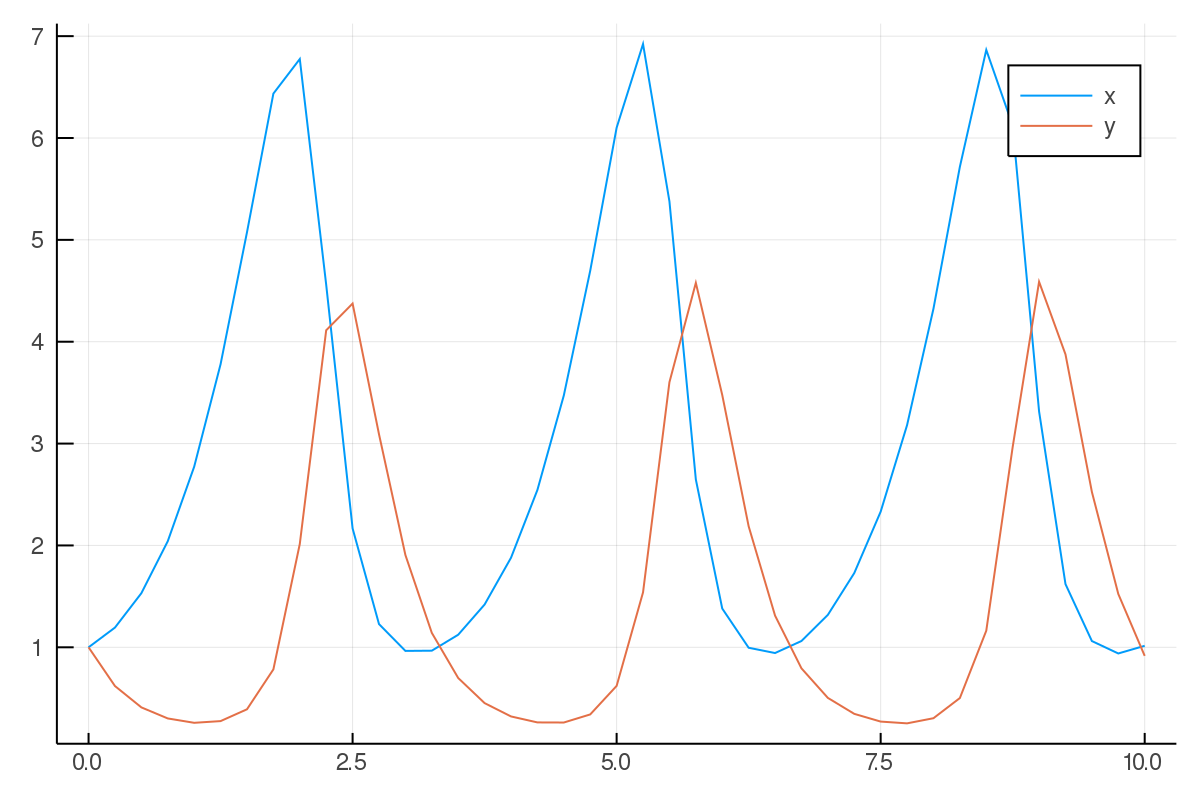
\includegraphics[width=.9\linewidth]{./.ob-jupyter/b27be8bcde0ff347ce1871cc1ed5426c5cf57422.png}
\end{center}


And, for comparison, a plot of the Euler solution with a much smaller step
size:
\begin{minted}[frame=lines,linenos=true,mathescape,breaklines=true]{julia}
ts_, us_ = solve(lotka_volterra, start, dt=0.01, tmin=0.0, tmax=10.0, step=euler_step)
us_ = hcat([[u[i] for u in us_] for i in 1:2]...)
plot(ts_, us_, format=:png, dpi=200, labels=["x", "y"])
\end{minted}

\begin{center}
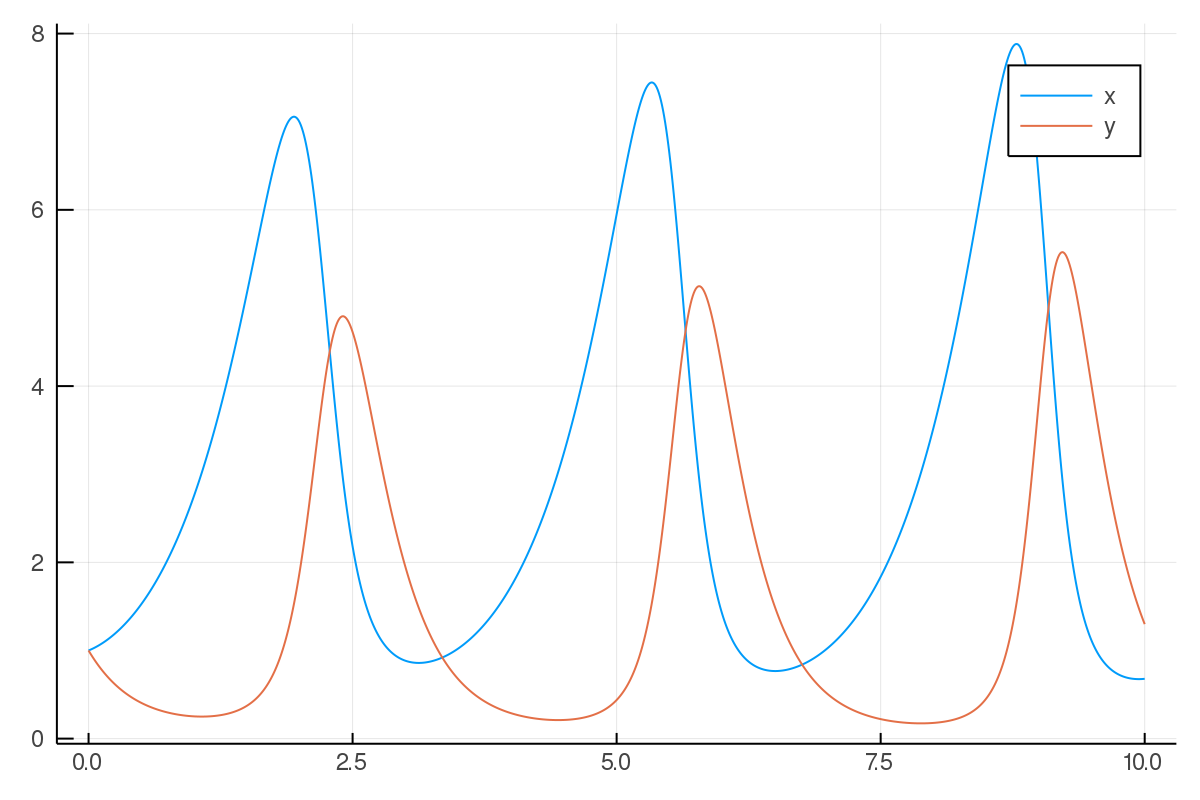
\includegraphics[width=.9\linewidth]{./.ob-jupyter/dc7fae37e0dfe8d7652748ee8251f0030fd7b5cd.png}
\end{center}

Pretty close!

\subsection{Part 2: Forward Sensitivity}
\label{sec:orgeb9559c}

We want to compute \(\frac{\partial \uv}{\partial \pv}|_t\), the sensitivity of the solution to the parameters at some time \(t\).
(Note that \(\frac{\partial \uv}{\partial \pv}\) is a 2-by-4 matrix in the case of the lotka-volterra equations.)

We have:

$$\frac{\partial}{\partial t}\frac{\partial \uv}{\partial \pv}
   =\frac{\partial \fv}{\partial \uv}\frac{\partial \uv}{\partial \pv}+\frac{\partial \fv}{\partial \pv}$$

So we have a (matrix) differential equation in \(\frac{\partial \uv}{\partial \pv}\), which we can integrate along with \(\uv\) in our solver.

m rows, n cols

Now we have:

$$\frac{\partial \fv}{\partial \uv}
   =\left(\begin{array}{cccc}
     \frac{\partial f_{1}}{\partial u_{1}} & \frac{\partial f_{1}}{\partial u_{2}} & \cdots & \frac{\partial f_{1}}{\partial u_{s}}\\
     \frac{\partial f_{2}}{\partial u_{1}} & \frac{\partial f_{2}}{\partial u_{2}} & \cdots & \frac{\partial f_{2}}{\partial u_{s}}\\
     \cdots & \cdots & \cdots & \cdots\\
     \frac{\partial f_{s}}{\partial u_{1}} & \frac{\partial f_{s}}{\partial u_{2}} & \cdots & \frac{\partial f_{s}}{\partial u_{s}}
   \end{array}\right)$$

$$\frac{\partial \fv}{\partial \pv}
   =\left(\begin{array}{cccc}
     \frac{\partial f_{1}}{\partial p_{1}} & \frac{\partial f_{1}}{\partial p_{2}} & \cdots & \frac{\partial f_{1}}{\partial p_{s}}\\
     \frac{\partial f_{2}}{\partial p_{1}} & \frac{\partial f_{2}}{\partial p_{2}} & \cdots & \frac{\partial f_{2}}{\partial p_{s}}\\
     \cdots & \cdots & \cdots & \cdots\\
     \frac{\partial f_{s}}{\partial p_{1}} & \frac{\partial f_{s}}{\partial p_{2}} & \cdots & \frac{\partial f_{s}}{\partial p_{s}}
   \end{array}\right)$$

Plugging in:

\begin{align}
   \frac{dx}{dt} &= \alpha x - \beta x y\\
   \frac{dy}{dt} &= - \gamma y + \delta x y\\
   \end{align}

Gives:

\begin{align}
    \frac{\partial \fv}{\partial \uv}&=\left(\begin{array}{cc}
     \frac{\partial }{\partial x} (\alpha x - \beta x y) & \frac{\partial}{\partial y} (\alpha x - \beta x y) \\
     \frac{\partial }{\partial x} (- \gamma y + \delta x y) & \frac{\partial}{\partial y} (- \gamma y + \delta x y) \\
   \end{array}\right)\\
   &=\left(\begin{array}{cc}
     \alpha - \beta y & -\beta x \\
     \delta y       & -\gamma + \delta x \\
   \end{array}\right)
\end{align}

and:

\begin{align}\frac{\partial \fv}{\partial \pv} &=\left(\begin{array}{cccc}
   \frac{\partial }{\partial \alpha} (\alpha x - \beta x y) & \frac{\partial }{\partial \beta} (\alpha x - \beta x y) &
   \frac{\partial }{\partial \gamma} (\alpha x - \beta x y) & \frac{\partial }{\partial \delta} (\alpha x - \beta x y)\\
   \frac{\partial }{\partial \alpha} (-\gamma y + \delta x y) & \frac{\partial }{\partial \beta} (-\gamma y + \delta x y) &
   \frac{\partial }{\partial \gamma} (-\gamma y + \delta x y) & \frac{\partial }{\partial \delta} (-\gamma y + \delta x y)\\
   \end{array}\right)\\
   &=\left(\begin{array}{cccc}
   x & -x y & 0 & 0 \\
   0 & 0 & -y & xy \\
   \end{array}\right)\end{align}

Great. Now, let's define some functions to wrap this sensitivity matrix into / out of a vector:

\begin{minted}[frame=lines,linenos=true,mathescape,breaklines=true]{julia}
function wrap_sensitivities(u, s)
    return vcat(u, reshape(s, 8))
end
function unwrap_sensitivities(us)
    u = us[1:2]
    s = reshape(us[3:10], (2, 4))
    u, s
end
u = [1., 2]
s = [1. 2 3 4; 5 6 7 8]
us = wrap_sensitivities(u, s)
u_, s_ = unwrap_sensitivities(us)

@assert u == u_ && s == s_
\end{minted}

And a function to operate on those vectors:

\begin{minted}[frame=lines,linenos=true,mathescape,breaklines=true]{julia}
function lotka_volterra_sens(_t, us, p)
    u, s = unwrap_sensitivities(us)

    x = u[1]
    y = u[2]

    α = p[1]
    β = p[2]
    γ = p[3]
    δ = p[4]

    dx = α*x - β*x*y
    dy = - γ*y + δ*x*y

    du = @SVector [dx, dy]

    dfdu = @SMatrix [(α - β * y) (-β * x); (δ * y) (-γ + δ * x)]
    dfdp = @SMatrix [x (-x*y) 0 0; 0 0 (-y) (x*y)]

    ds = dfdu * s + dfdp

    wrap_sensitivities(du, ds)
end
\end{minted}

\begin{minted}[frame=lines,linenos=true,mathescape,breaklines=true]{julia}
lotka_volterra_sens (generic function with 1 method)
\end{minted}


Now we can solve for \(\uv\), along with the sensitivities:

\begin{minted}[frame=lines,linenos=true,mathescape,breaklines=true]{julia}
start_sensitivities = @SMatrix [0. 0 0 0; 0 0 0 0]
start_ = wrap_sensitivities(start, start_sensitivities)
p = @SVector [1.5, 1.0, 3.0, 1.0]

ts, us = solve((t, u) -> lotka_volterra_sens(t, u, p), start_, dt=0.25, tmin=0.0, tmax=10.0)
xy = hcat([[u[i] for u in us] for i in 1:2]...)

u_names = ["x", "y"]
p_names = ["alpha", "beta", "gamma", "delta"]

ss = hcat([[unwrap_sensitivities(u)[2][i,j] for u in us] for j in 1:4 for i in 1:2]...)
labels = ["d$(u_names[i])/d$(p_names[j])" for j in 1:4 for i in 1:2]
plot(ts, ss, format=:png, dpi=200, labels=labels)
\end{minted}

\begin{center}
\includegraphics[width=.9\linewidth]{./.ob-jupyter/8c0de185a3d547b2ebef56a15e6898b563b8487d.png}
\end{center}

Quite a tangle.

We can compare this to the results found by \texttt{ForwardDiff}:

\begin{minted}[frame=lines,linenos=true,mathescape,breaklines=true]{julia}
using ForwardDiff

function solve_p(p :: SVector)
    ts, us = solve((t, u) -> lotka_volterra(t, u, p=p), start, dt=0.25, tmin=0.0, tmax=10.0)
    xy = hcat([[u[i] for u in us] for i in 1:2]...)
    return xy
end

xy = solve_p(p)
ss_ = ForwardDiff.jacobian(solve_p, p)
ss_ = reshape(ss_, (:, 2, 4))
@assert all(abs.(ss_ - reshape(ss, (:, 2, 4))) .< .0001)
\end{minted}

So our sensitivity algorithm seems to work correctly.

\subsection{Part 3: Parameter Estimation}
\label{sec:orgd17c994}
We can compute the gradient of the loss with respect to the parameters:

$$\frac{dl}{d\pv} = \frac{dl}{d\uv} \frac{d\uv}{d\pv}$$

Note the multiplication order; the gradient is a row vector.
We have \(l = (x - x^*)^2 + (y - y^*)^2\), where \(x^*\) is the target value of \(x\) at a point. Therefore:

$$\frac{dl}{d\uv} = \left(\begin{array}{cc}\frac{dl}{dx} & \frac{dl}{dy}\end{array}\right)
   = \left(\begin{array}{cc} 2(x-x^*) & 2(y-y^*) \end{array}\right)$$

Which we can sum over all the data points.

\begin{minted}[frame=lines,linenos=true,mathescape,breaklines=true]{julia}

function compute_grads(p :: SVector, training_xy :: Array)
    _, us = solve((t, u) -> lotka_volterra_sens(t, u, p), start_, dt=0.25, tmin=0.0, tmax=10.0)

    dldp = @SMatrix [0. 0 0 0]
    for i in 1:(size(us)[1])
        ut = training_xy[i, :]
        u, s = unwrap_sensitivities(us[i])

        x, y = u
        xt, yt = ut

        dldu = @SMatrix [2(x-xt) 2(y-yt)]
        dldp += dldu * s
    end

    # mean over training data set
    dldp /= size(us)[1]

    reshape(dldp, 4)
end

p_ = @SVector [1.2, 0.8, 2.8, 0.8]
sens_grads = compute_grads(p_, xy)
()
\end{minted}

Let's again compare it to the results from ForwardDiff:

\begin{minted}[frame=lines,linenos=true,mathescape,breaklines=true]{julia}
function compute_loss(p :: SVector, training_xy :: Array)
    _, us = solve((t, u) -> lotka_volterra(t, u, p=p), start, dt=0.25, tmin=0.0, tmax=10.0)

    loss = 0.0
    for i in 1:size(us)[1]
        xt, yt = us[i]
        x, y = training_xy[i, :]
        loss_i = (x - xt)^2 + (y - yt)^2
        loss += loss_i
    end

    loss /= size(us)[1]

    loss
end

fd_grads = ForwardDiff.gradient((p) -> compute_loss(p, xy), p_)
@assert all(abs.(fd_grads - sens_grads) .< .1)
\end{minted}

Seems reasonable. Now, let's fit the model:

\begin{minted}[frame=lines,linenos=true,mathescape,breaklines=true]{julia}
function fit_parameters(p0 :: SVector, training_xy :: Array; steps = 1000, alpha = 0.001)
    p = p0
    intermediates = typeof(p)[]

    for _ in 1:steps
        push!(intermediates, p)
        dldp = compute_grads(p, training_xy)
        p = p - dldp * alpha
    end

    p, intermediates
end

p_fit, intermediates = fit_parameters(p_, xy)
p_fit
\end{minted}

\begin{minted}[frame=lines,linenos=true,mathescape,breaklines=true]{julia}
4-element SArray{Tuple{4},Float64,1,4} with indices SOneTo(4):
 1.5226861718402038
 1.01427426674589  
 2.9340399220263254
 0.9768262463926147
\end{minted}


That's close to the correct values of \([1.5, 2.0, 3.0, 1.0]\).

We can plot it:

\begin{minted}[frame=lines,linenos=true,mathescape,breaklines=true]{julia}
function plot_compare(p_fit, title)
    ts, us = solve((t, u) -> lotka_volterra(t, u, p=p), start, dt=0.25, tmin=0.0, tmax=10.0)
    us = hcat([[u[i] for u in us] for i in 1:2]...)
    ts_fit, us_fit = solve((t, u) -> lotka_volterra(t, u, p=p_fit), start, dt=0.25, tmin=0.0, tmax=10.0)
    us_fit = hcat([[u[i] for u in us_fit] for i in 1:2]...)
    plot(ts, hcat(us, us_fit), format=:png, dpi=200, labels=["x", "y", "x*", "y*"], title=title)
end
plot_compare(p_fit, "comparison")
\end{minted}

\begin{center}
\includegraphics[width=.9\linewidth]{./.ob-jupyter/459d014f8c4878cf93f16375cdb8cfdc4a1665a0.png}
\end{center}

The solutions overlay nearly perfectly, even if the parameters are slightly off. More data points would let the parameters get even closer.

We can also plot the fit of the data over the course of training:

\begin{minted}[frame=lines,linenos=true,mathescape,breaklines=true]{julia}
@gif for i in 1:3:330
    plot_compare(intermediates[i], "fit: step $i")
end
\end{minted}

Link to the gif: \url{https://i.imgur.com/YSYEMTI.mp4}

\section{Problem 2: Bandwidth Maximization}
\label{sec:org792ecfd}
Here's the code:

\begin{minted}[frame=lines,linenos=true,mathescape,breaklines=true]{julia}
using Distributed
using MPI
using Statistics

MPI.Init()
comm = MPI.COMM_WORLD
my_rank = MPI.Comm_rank(comm)
n_procs = MPI.Comm_size(comm)
root = 0

max_n = 30 # ~1 GB
evals = 10

arr = zeros(Int8, 2^max_n)

times = zeros(Float64, max_n, evals)

hostname = chomp(read(`hostname`, String))

function send(n)
    viewed = @view arr[1:2^n]
    MPI.Send(viewed, 0, 0, comm)
    ()
end

function timerecv(n)
    viewed = @view arr[1:2^n]

    start = time_ns()
    MPI.Recv!(viewed, 1, 0, comm)
    end_ = time_ns()

    float(end_ - start) / 10^9 # in seconds
end

if my_rank == 0
    print("I'm the leader! on $hostname\n")

    # jit
    timerecv(0)

    for n in 1:max_n
        print("$n : ")
        for eval in 1:evals
            times[n, eval] = timerecv(n)
            print(".")
        end
        print("\n")
    end
    avg = mean(times, dims=2)
    print("\n\n$avg\n")
else
    # jit
    send(0)

    for n in 1:max_n
        for eval in 1:evals
            send(n)
        end
    end

    print("I'm the disciple! on $hostname\n")
end
\end{minted}

Note that I use \texttt{@view} + pre-compile my timing function to avoid costs from memory allocation and JIT respectively.

Results for 1 node:

\begin{minted}[frame=lines,linenos=true,mathescape,breaklines=true]{julia}
times = [4.7846e-6, 3.1569e-6, 3.0419e-6, 3.2474e-6, 3.1628e-6, 3.2524e-6, 2.4623e-6, 1.5921e-6, 1.6476e-6, 1.8483e-6, 1.9716e-6, 3.6974e-6, 4.2129e-6, 6.1383e-6, 9.4885e-6, 3.76671e-5, 4.15329e-5, 7.30508e-5, 0.000122126, 0.000233082, 0.000460704, 0.000914118, 0.00182519, 0.00378303, 0.00842342, 0.01682, 0.0302923, 0.0603868, 0.122339, 0.239431]
message_size = 2 .^ Array(1:30)
bandwidth = message_size ./ times

plot(message_size, bandwidth, format=:png, dpi=:200, xlabel="message size (bytes)", ylabel="bandwidth (bytes / s)",
     xscale=:log10, yscale=:log10, title="message size vs bandwidth, 1 node")
\end{minted}

\begin{center}
\includegraphics[width=.9\linewidth]{./.ob-jupyter/bbcebf0b041fac8d4931a822376ca3665eca868c.png}
\end{center}

\begin{minted}[frame=lines,linenos=true,mathescape,breaklines=true]{julia}
times = [4.99197e-5, 3.083e-6, 5.9434e-6, 3.0175e-6, 5.4554e-6, 5.0184e-6, 5.2316e-6, 5.7617e-6, 1.0404e-5, 1.36927e-5, 1.52306e-5, 1.84061e-5, 2.08266e-5, 2.49751e-5, 0.000123629, 0.000468794, 0.00131264, 0.00243091, 0.00467664, 0.00910919, 0.0179756, 0.0356573, 0.0710337, 0.142121, 0.283833, 0.566846, 1.13436, 2.2664, 4.53212, 9.06214]
message_size = 2 .^ Array(1:30)
bandwidth = message_size ./ times

plot(message_size, bandwidth, format=:png, dpi=:200, xlabel="message size (bytes)", ylabel="bandwidth (bytes / s)",
     xscale=:log10, yscale=:log10, title="message size vs bandwidth, 2 nodes")
\end{minted}

\begin{center}
\includegraphics[width=.9\linewidth]{./.ob-jupyter/ad006190492c0b7537e3455aca4d016cd162d287.png}
\end{center}

The minimal latency in the 1-node case was on the order of a microsecond, and in the 2-node case 10 microseconds; very fast. Both cases saturate the
link with messages of size \(~10^5\) bytes. We see that small messages need to encapsulate orders of magnitude more computation to be as efficient as
large messages.
\end{document}
